\subsection{Especificación del Diseño}
\subsubsection{Arquitectura y entorno tecnológico del proyecto}
\paragraph{Arquitectura del software}
La arquitectura del software del modelo está compuesta por cuatro capas principales: 
la capa del modelo, la capa del estado compuesto por un grafo, la capa del 
environment y la capa de ejecución. Se puede ver un diagrama de la arquitectura en la
Figura \ref{fig:layers}.

\begin{itemize}
    \item \textbf{Capa de ejecución:} Esta capa se encarga de ejecutar todo el ecosistema
    del modelo. En nuestro caso es ejecutada por Python 3.10.6 \cite{C8d} y ofrece la versatilidad de
    poder ejecutar el modelo ya sea en un entorno local o en la nube. 
    \item \textbf{Capa del environment:} Esta capa se encarga de generar el entorno en el que se
    ejecutará el modelo. Cuando se va a resolver un problema de scheduling, el entorno
    prepara todo lo necesario para que el modelo pueda interactuar con el problema y le
    proporciona toda la información necesaria para que pueda tomar decisiones.
    \item \textbf{Capa del estado:} Esta capa se encarga de representar el estado del problema
    mediante un grafo. El grafo representa todas las operaciones que se deben ejecutar y
    las restricciones que existen entre ellas.
    \item \textbf{Capa del modelo:} Esta capa se encarga de resolver el problema de scheduling
    mediante un modelo de Deep Learning. El modelo recibe como entrada el grafo del
    estado y genera como salida una asignación de las operaciones a los recursos. 
\end{itemize}

\begin{figure}[ht]
    \centering
    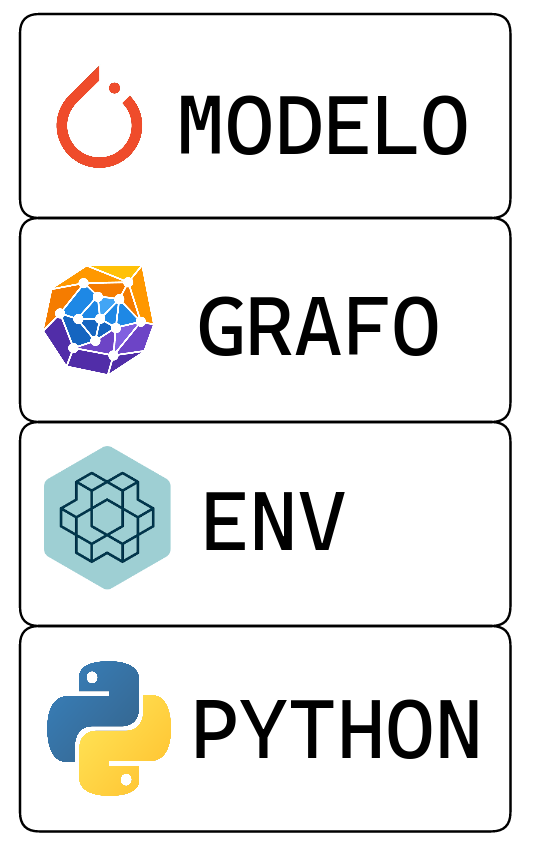
\includegraphics[scale=0.27]{layers.png}
    \caption{Capas de la arquitectura}
    \label{fig:layers}
\end{figure}


\paragraph{Despliegue fisico}
La visualización de los resultados es una parte crítica e importante del proceso. Permite 
a los usuarios finales entender y analizar los datos de una manera más efectiva.  
Sin embargo, es importante destacar que esta parte del proyecto es 
estrictamente opcional y dependerá de las necesidades concretas del caso de uso. 
Si bien la visualización del problema puede ser extremadamente útil algunos casos, puede que no sea 
relevante o necesaria en otros. Por lo tanto, se debe evaluar cuidadosamente la necesidad de 
esta visualización antes de implementarla, ya que puede ser un proceso costoso y 
requerir mucho tiempo.\medskip

\begin{figure}[ht]
    \centering
    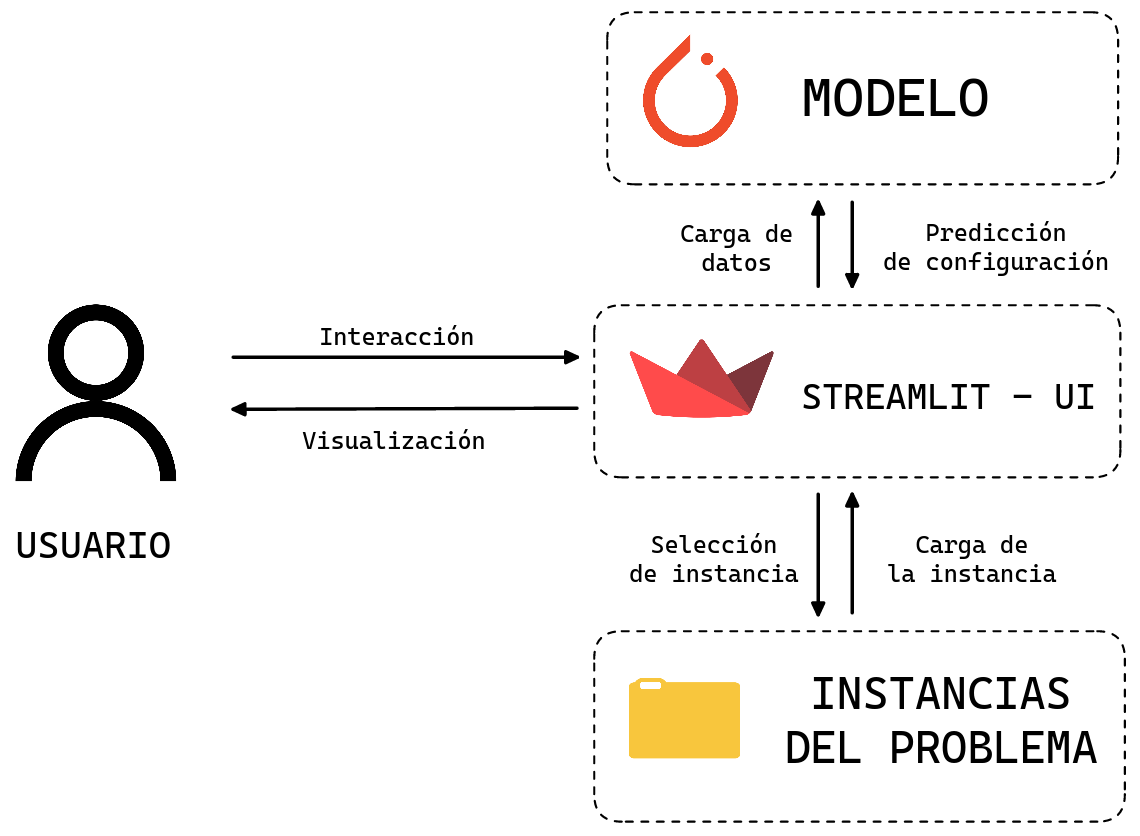
\includegraphics[scale=0.25]{deploy.png}
    \caption{Arquitectura física}
    \label{fig:despliegue}
\end{figure}

En este proyecto en particular, se ha optado por se crear una aplicación web en Streamit \cite{Streamlit} 
desde la cual mediante una llamada al modelo generar un gráfico Gantt en el que se podrá
visualizar todas las operaciones y sus respectivas asignaciones y tiempos de ejecución.
En la Figura \ref{fig:despliegue} se puede ver un diagrama del despliegue físico del modelo.
La aplicación sirve como intermediario entre el usuario y el modelo, para ello extrae las
diferentes configuraciones de problemas desde una carpeta en la que se encuentran los 
archivos. Lo importante de esta distribución es que permite una gran versatilidad a la hora
de ejecutar el modelo, ya que se podría mover la ejecución del modelo a un microservicio
externo que se encargue de ejecutar el modelo y devolver los resultados a la aplicación web.
Para ver más información sobre la aplicación web, se puede consultar el apartado de manual
de usuario donde se explica con más detalle. 

\subsubsection{Descripcion del diseño}
Uno de los diseños más comúnmente utilizados para resolver problemas de Machine learning
es el uso de sistemas de pipelines. Estos sistemas escapan del paradigma tradicional de
programación secuencial y se basan en la idea de que el problema se puede resolver
mediante la composición de una serie de pasos o etapas. Cada etapa se encarga de realizar
una tarea específica y se comunica con las demás mediante un sistema de colas. De esta
manera, se puede lograr un sistema altamente escalable y flexible. Además, se puede
reutilizar cada etapa para diferentes pipelines o enlazar diferentes pipelines para
conseguir uno más complejo. Otra de las ventajas de este diseño es que permite
abstraer la implementación de cada etapa, lo que permite que cada una de ellas se pueda
mejorar o cambiar sin afectar al resto de ellas, siempre y cuando se mantenga la
interfaz de comunicación.

\subsubsection{Modelo de diseño}
\begin{figure}[ht]
    \centering
    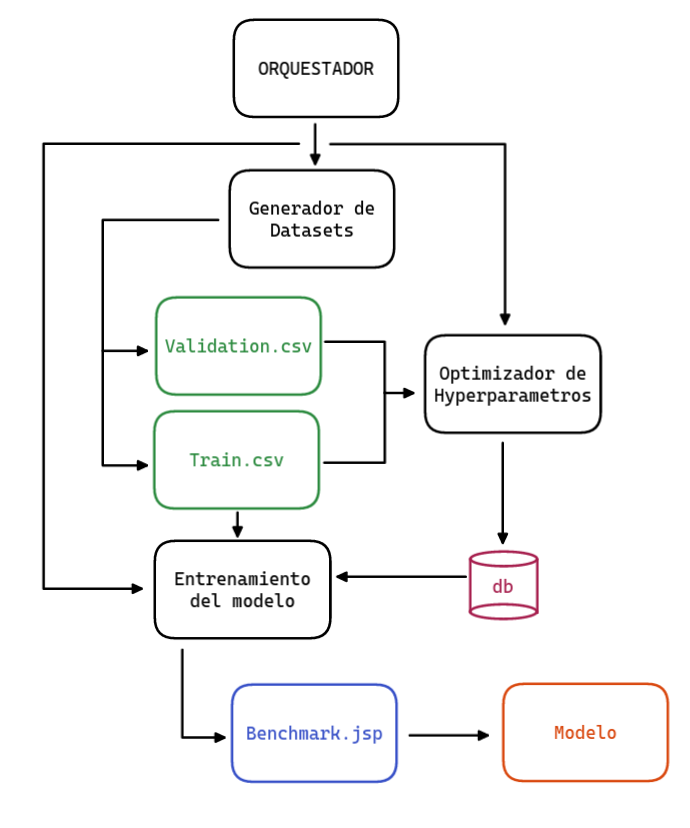
\includegraphics[scale=0.35]{disenio.png}
    \caption{Diseño del sistema}
    \label{fig:desing}
\end{figure}

En la figura \ref{fig:desing} se puede ver al completo las diferentes etapas que componen
el sistema. Podemos identificar las siguientes etapas:
\begin{itemize}
    \item \textbf{Generador de datasets: } Este pipeline se encarga de generar los datasets
    que se utilizarán para entrenar el modelo y para su validación. Estos son dos .csv que
    contienen las diferentes configuraciones de problemas que se van a utilizar. Y que se
    utilizan para el resto de pipelines.
    \item \textbf{Optimizador de hiperparámetros: } Este pipeline se encarga de optimizar
    los hiperparámetros del modelo. Para ello utiliza el dataset de validación como una
    forma de medir el rendimiento del modelo. El objetivo de este pipeline es encontrar
    la configuración de hiperparámetros que mejor se adapte al problema. Estos resultados
    se guardan en una base de datos Sqlite3.
    \item \textbf{Entrenamiento del modelo: } Este pipeline se encarga de entrenar el modelo
    con la configuración de hiperparámetros que ha sido almacenada en la base de datos por el
    anterior pipeline. El modelo se entrena con el dataset de entrenamiento pero antes de
    guardar el modelo se evalúa con el benchmark para comprobar el rendimiento real del modelo.
\end{itemize} 

Todas estas etapas son gestionadas por el orquestador de pipelines. Este se encarga de
gestionar el flujo de datos entre las diferentes etapas y de asegurar que se ejecutan en
el orden correcto y que se cumplen las dependencias entre ellas.